\documentclass[10pt]{article}
\usepackage[utf8]{inputenc}
\usepackage[T1]{fontenc}
\usepackage{graphicx}
\usepackage{lipsum}
\usepackage{geometry}
\usepackage{titlesec}
\usepackage{times}
\usepackage{hyperref}
\usepackage{amsmath}
\usepackage[linesnumbered,ruled,vlined]{algorithm2e}
\usepackage{listings}
\usepackage{color}
\usepackage{fancyhdr}
\geometry{a4paper, margin=0.75in}
%\geometry{left=2.5cm, right=2.5cm, top=2.5cm, bottom=2.5cm}
\pagestyle{fancy}
\fancyhf{} % Clear all header and footer fields
\fancyhead[L]{<NEAT-Pong>}
\fancyhead[C]{Artificial Intelligence} % Centrally aligned header
\fancyhead[R]{<Project Report>}
\fancyfoot[C]{\thepage} % Centrally aligned footer with page number
\usepackage{xcolor}

% Define colors for code listing
\definecolor{codegreen}{rgb}{0,0.6,0}
\definecolor{codegray}{rgb}{0.5,0.5,0.5}
\definecolor{codepurple}{rgb}{0.58,0,0.82}
\definecolor{backcolour}{rgb}{0.95,0.95,0.92}

% Setup the style for code listing
\lstdefinestyle{mystyle}{
    backgroundcolor=\color{backcolour},   
    commentstyle=\color{codegreen},
    keywordstyle=\color{magenta},
    numberstyle=\tiny\color{codegray},
    stringstyle=\color{codepurple},
    basicstyle=\ttfamily\footnotesize,
    breakatwhitespace=false,         
    breaklines=true,                 
    captionpos=b,                    
    keepspaces=true,                 
    numbers=left,                    
    numbersep=5pt,                  
    showspaces=false,                
    showstringspaces=false,
    showtabs=false,                  
    tabsize=2
}

\lstset{style=mystyle}

\begin{document}
\begin{titlepage}
    \centering
    \vspace{3.5cm}
    
\includegraphics[width=0.5\textwidth]{FAST.png}\par\vspace{1cm}
    
\includegraphics[width=0.5\textwidth]{NU-logo.jpg}\par\vspace{1cm}
    \vspace{1.5cm}
    {\scshape\Huge\textbf {Project Report} \par}
    \vspace{1.5cm}
    % {\scshape\Huge\textbf {AI-Controlled Pong Game Using NEAT Algorithm\\} \par}
    % {\scshape\Large Version 1.0 \par}
    \vspace{1cm}
    {\scshape\LARGE\textbf {Lecturer Ms. Mafaza Mohi (BCS-6E)}\\ \par}
    \vspace{1cm}
    {\scshape\LARGE\textbf {Instructor Mr. Muhammad Osaid (BCS-6E)}\\ \par}
    \vspace{1cm}
    {\scshape\LARGE\textbf {Artificial Intelligence (AI-2002/AL-2002)} \par}
    \vspace{1.25cm}
    \vspace{1.25cm}
    \begin{itemize}
    \item {\scshape\LARGE Muhammad Hamza (K21-4579) \par}
    \vspace{0.12cm}
    \item {\scshape\LARGE Muhammad Salar (K21-4619) \par}
    \vspace{0.12cm}
    \item {\scshape\LARGE Bilal Shakeel (K21-4874) \par}
    \end{itemize}
    \vfill   
    {Foundation of Advancement of Science and Technology \par}
    {National University of Computer and Emerging Sciences \par}
    {Department of Computer Science \par}
    {Karachi, Pakistan \par}
\end{titlepage}

\tableofcontents
\title{AI-Controlled Pong Game Using NEAT Algorithm}
\author{Muhammad Salar, Muhammad Hamza, Bilal Shakeel}
\date{\today}
\maketitle

\begin{abstract}
This report presents the development of an AI-driven Pong game using the NeuroEvolution of Augmenting Topologies (NEAT) algorithm. The aim was to transcend the conventional Pong experience by introducing a self-learning AI opponent, thereby offering a dynamic and progressively challenging gameplay experience.
\end{abstract}

\section{Introduction}
Pong, the quintessential arcade game, has been a cornerstone in the gaming industry. This project introduces a novel twist by integrating an AI opponent powered by the NEAT algorithm, capable of competing against human players and other AI entities with remarkable efficacy.

\section{Background}
The classic Pong game involves two players maneuvering paddles to volley a ball across the screen. The simplicity of the game, while charming, often leads to a static and predictable experience. This project aims to revitalize the Pong experience by incorporating an AI that not only competes but evolves.

\section{Problem Definition}
The static nature of traditional Pong AI creates a monotonous experience for players. This project addresses the need for a dynamic opponent that can adapt its strategies to the evolving gameplay, thereby enhancing player engagement.

\section{Proposed Methodology}
The project employs Python and Pygame to simulate the Pong environment, establishing the foundational rules, paddle mechanics, and ball dynamics. The NEAT algorithm is at the heart of the AI development, enabling the evolution of neural networks that act as the AI players. These networks undergo training through interactive gameplay, with their efficacy gauged by their competitive prowess.

\section{System Architecture}
The system is structured around the \texttt{PongGame} class, which orchestrates the game's logic and the AI's developmental cycle. Functions like \texttt{test\_ai}, \texttt{train\_ai}, \texttt{move\_ai\_paddles}, and \texttt{calculate\_fitness} are integral to the AI's learning mechanism. The system also incorporates a checkpoint management system to preserve the evolutionary progress of the AI.

\section{Distinctive Features}
\begin{itemize}
    \item \textbf{Dynamic Adaptation}: The AI dynamically adjusts its strategies in response to the ball's movement, ensuring a fluid and responsive gameplay.
    \item \textbf{Continuous Learning}: The AI's ability to learn from each session guarantees a consistently escalating challenge for players.
\end{itemize}

\section{Technological Stack}
\begin{itemize}
    \item \textbf{Python}: The primary language for crafting the game and AI logic.
    \item \textbf{Pygame}: The framework for rendering the 2D game environment and handling user interactions.
    \item \textbf{NEAT-Python}: The chosen library for implementing the NEAT algorithm.
    \item \textbf{Development Environment}: The use of an IDE such as Visual Studio Code streamlined the development process.
\end{itemize}

\section{Conclusion}
The project culminates in the creation of an AI-driven Pong game that elevates the player's experience by introducing a real-time learning and adapting AI opponent. This advancement significantly enriches the Pong gameplay, marking a substantial contribution to the domains of game development and artificial intelligence.


\section{Future Directions}
Prospective developments include the introduction of multiplayer capabilities, the refinement of AI learning algorithms, and the incorporation of intricate game elements to further enhance the gaming experience.

\section{Acknowledgments}
The project owes its success to the collective efforts of the contributors and the invaluable resources provided by the open-source community.

\section{References} A comprehensive list of references is included, citing the sources of information, libraries, and tools used throughout the project’s development.
\begin{itemize} 
    \item Python Documentation: \url{https://docs.python.org/3/}
    \item Pygame Documentation: \url{https://www.pygame.org/docs/} 
    \item NEAT-Python Documentation: \url{https://neat-python.readthedocs.io/en/latest/index.html#} 
    \item Efficient Evolution of Neural Network Topologies: \url{https://nn.cs.utexas.edu/downloads/papers/stanley.cec02.pdf}
    \item Pong Game Documentation: \url{https://pysdl2.readthedocs.io/en/latest/tutorial/pong.html#}  
    \item Visual Studio Code Documentation: \url{https://code.visualstudio.com/docs} 
\end{itemize}

\newpage

\section{Screenshots}
\begin{figure}[h]
    \centering
    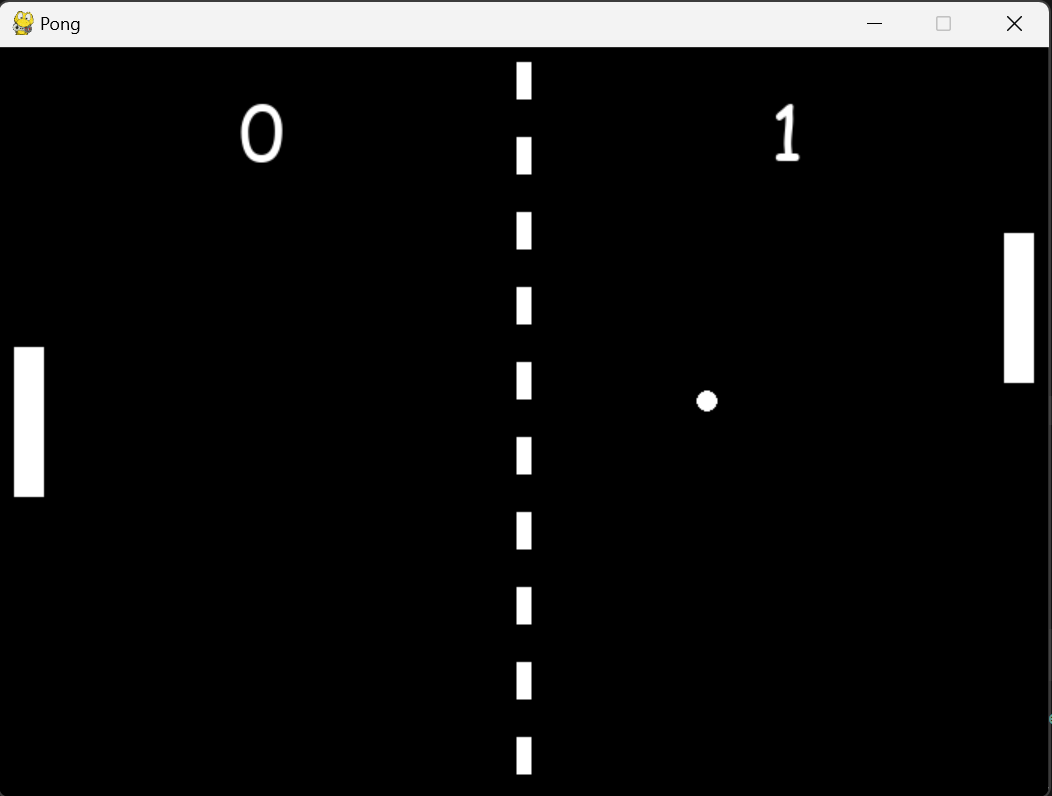
\includegraphics[width=0.8\textwidth]{Game.png} 
    \caption{Game Window}
    \label{fig:example}
\end{figure}
\begin{figure}[h]
    \centering
    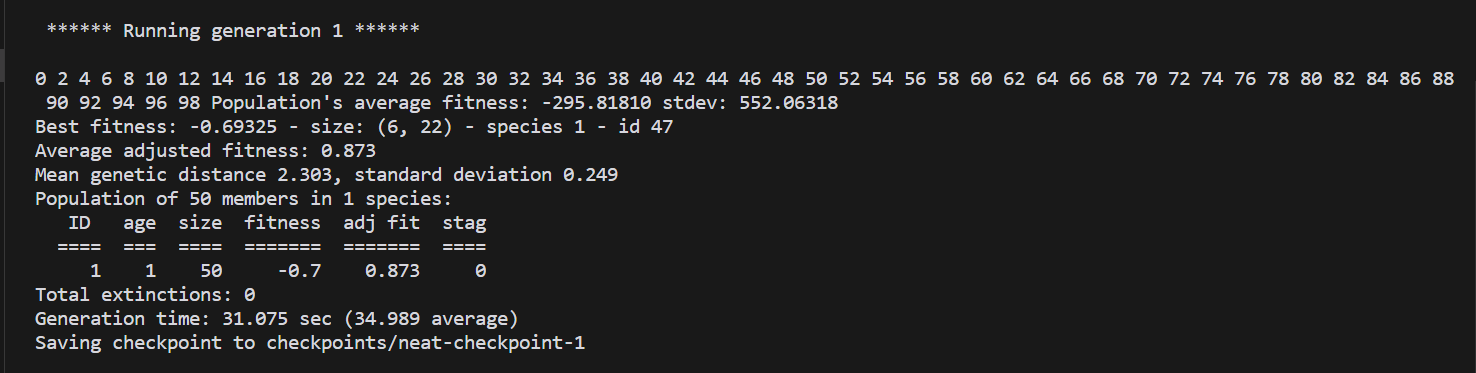
\includegraphics[width=0.8\textwidth, height=0.22\textheight]{Training.png} 
    \caption{Training Model}
    \label{fig:example}
\end{figure}

\newpage

\section*{\centering{Appendix}}
Included is the complete source code for the \texttt{main.py}, \texttt{paddle.py}, \texttt{game.py}, and \texttt{ball.py} files, illustrating the implementation details of the Pong game and the NEAT algorithm's application in AI training and testing, along with the configuration file \texttt{config.txt}.

\begin{lstlisting}[language=Python, caption=main.py code]
from pong import Game
import pygame
import neat
import os
import time
import pickle
import glob

class PongGame:
    def __init__(self, window, width, height):
        self.game = Game(window, width, height)
        self.ball = self.game.ball
        self.left_paddle = self.game.left_paddle
        self.right_paddle = self.game.right_paddle

    def test_ai(self, net):
        clock = pygame.time.Clock()
        run = True
        while run:
            clock.tick(144)
            game_info = self.game.loop()
            for event in pygame.event.get():
                if event.type == pygame.QUIT:
                    run = False
                    break
            output = net.activate((self.right_paddle.y, abs(self.right_paddle.x - self.ball.x), self.ball.y))
            decision = output.index(max(output))
            if decision == 1:
                self.game.move_paddle(left=False, up=True)
            elif decision == 2:
                self.game.move_paddle(left=False, up=False)
            keys = pygame.key.get_pressed()
            if keys[pygame.K_w]:
                self.game.move_paddle(left=True, up=True)
            elif keys[pygame.K_s]:
                self.game.move_paddle(left=True, up=False)
            self.game.draw(draw_score=True)
            pygame.display.update()

    def train_ai(self, genome1, genome2, config, draw=False):
        run = True
        start_time = time.time()
        net1 = neat.nn.FeedForwardNetwork.create(genome1, config)
        net2 = neat.nn.FeedForwardNetwork.create(genome2, config)
        self.genome1 = genome1
        self.genome2 = genome2
        max_hits = 50
        while run:
            for event in pygame.event.get():
                if event.type == pygame.QUIT:
                    return True
            game_info = self.game.loop()
            self.move_ai_paddles(net1, net2)
            if draw:
                self.game.draw(draw_score=False, draw_hits=True)
            pygame.display.update()
            duration = time.time() - start_time
            if game_info.left_score == 1 or game_info.right_score == 1 or game_info.left_hits >= max_hits:
                self.calculate_fitness(game_info, duration)
                break
        return False

    def move_ai_paddles(self, net1, net2):
        players = [(self.genome1, net1, self.left_paddle, True), (self.genome2, net2, self.right_paddle, False)]
        for (genome, net, paddle, left) in players:
            output = net.activate((paddle.y, abs(paddle.x - self.ball.x), self.ball.y))
            decision = output.index(max(output))
            if decision == 0:
                genome.fitness -= 0.01
            elif decision == 1:
                valid = self.game.move_paddle(left=left, up=True)
            else:
                valid = self.game.move_paddle(left=left, up=False)
            if not valid:
                genome.fitness -= 1

    def calculate_fitness(self, game_info, duration):
        self.genome1.fitness += game_info.left_hits + duration
        self.genome2.fitness += game_info.right_hits + duration

def eval_genomes(genomes, config):
    width, height = 700, 500
    win = pygame.display.set_mode((width, height))
    pygame.display.set_caption("Pong")
    for i, (genome_id1, genome1) in enumerate(genomes):
        print(round(i/len(genomes) * 100), end=" ")
        genome1.fitness = 0
        for genome_id2, genome2 in genomes[min(i+1, len(genomes) - 1):]:
            genome2.fitness = 0 if genome2.fitness == None else genome2.fitness
            pong = PongGame(win, width, height)
            force_quit = pong.train_ai(genome1, genome2, config, draw=True)
            if force_quit:
                quit()

def find_latest_checkpoint():
    list_of_files = glob.glob('checkpoints/neat-checkpoint-*')
    if not list_of_files:
        return None
    latest_file = max(list_of_files, key=os.path.getctime)
    return latest_file

def run_neat(config, total_generations):
    latest_checkpoint = find_latest_checkpoint()
    if latest_checkpoint:
        generation_number = int(latest_checkpoint.split('-')[-1]) + 1
        if generation_number >= total_generations:
            print(f"{total_generations} generations completed. Skipping training.")
            return
        print(f"Resuming from checkpoint: {latest_checkpoint}")
        p = neat.Checkpointer.restore_checkpoint(latest_checkpoint)
    else:
        print("No checkpoints found. Starting new training session.")
        p = neat.Population(config)
    p.add_reporter(neat.StdOutReporter(True))
    stats = neat.StatisticsReporter()
    p.add_reporter(stats)
    p.add_reporter(neat.Checkpointer(1, filename_prefix='checkpoints/neat-checkpoint-'))
    winner = p.run(eval_genomes, total_generations - generation_number)
    with open("best.pickle", "wb") as f:
        pickle.dump(winner, f)

def test_best_network(config):
    with open("best.pickle", "rb") as f:
        winner = pickle.load(f)
    winner_net = neat.nn.FeedForwardNetwork.create(winner, config)
    width, height = 700, 500
    win = pygame.display.set_mode((width, height))
    pygame.display.set_caption("Pong")
    pong = PongGame(win, width, height)
    pong.test_ai(winner_net)

if __name__ == '__main__':
    local_dir = os.path.dirname(__file__)
    config_path = os.path.join(local_dir, 'config.txt')
    config = neat.Config(neat.DefaultGenome, neat.DefaultReproduction, neat.DefaultSpeciesSet, neat.DefaultStagnation, config_path)
    run_neat(config ,50)
    test_best_network(config)
\end{lstlisting}

\begin{lstlisting}[language=Python, caption=paddle.py code]
import pygame

class Paddle:
    VEL = 4
    WIDTH = 20
    HEIGHT = 100

    def __init__(self, x, y):
        self.x = self.original_x = x
        self.y = self.original_y = y

    def draw(self, win):
        pygame.draw.rect(win, (255, 255, 255), (self.x, self.y, self.WIDTH, self.HEIGHT))

    def move(self, up=True):
        if up:
            self.y -= self.VEL
        else:
            self.y += self.VEL

    def reset(self):
        self.x = self.original_x
        self.y = self.original_y
\end{lstlisting}

\begin{lstlisting}[language=Python, caption=game.py code]
from .paddle import Paddle
from .ball import Ball
import pygame
import random
pygame.init()

class GameInformation:
    def __init__(self, left_hits, right_hits, left_score, right_score):
        self.left_hits = left_hits
        self.right_hits = right_hits
        self.left_score = left_score
        self.right_score = right_score

class Game:
    SCORE_FONT = pygame.font.SysFont("comicsans", 50)
    WHITE = (255, 255, 255)
    BLACK = (0, 0, 0)
    RED = (255, 0, 0)

    def __init__(self, window, window_width, window_height):
        self.window_width = window_width
        self.window_height = window_height
        self.left_paddle = Paddle(10, self.window_height // 2 - Paddle.HEIGHT // 2)
        self.right_paddle = Paddle(self.window_width - 10 - Paddle.WIDTH, self.window_height // 2 - Paddle.HEIGHT//2)
        self.ball = Ball(self.window_width // 2, self.window_height // 2)
        self.left_score = 0
        self.right_score = 0
        self.left_hits = 0
        self.right_hits = 0
        self.window = window

    def _draw_score(self):
        left_score_text = self.SCORE_FONT.render(f"{self.left_score}", 1, self.WHITE)
        right_score_text = self.SCORE_FONT.render(f"{self.right_score}", 1, self.WHITE)
        self.window.blit(left_score_text, (self.window_width // 4 - left_score_text.get_width()//2, 20))
        self.window.blit(right_score_text, (self.window_width * (3/4) - right_score_text.get_width()//2, 20))

    def _draw_hits(self):
        hits_text = self.SCORE_FONT.render(f"{self.left_hits + self.right_hits}", 1, self.RED)
        self.window.blit(hits_text, (self.window_width // 2 - hits_text.get_width()//2, 10))

    def _draw_divider(self):
        for i in range(10, self.window_height, self.window_height//20):
            if i % 2 == 1:
                continue
            pygame.draw.rect(self.window, self.WHITE, (self.window_width//2 - 5, i, 10, self.window_height//20))

    def _handle_collision(self):
        ball = self.ball
        left_paddle = self.left_paddle
        right_paddle = self.right_paddle

        if ball.y + ball.RADIUS >= self.window_height:
            ball.y_vel *= -1
        elif ball.y - ball.RADIUS <= 0:
            ball.y_vel *= -1

        if ball.x_vel < 0:
            if ball.y >= left_paddle.y and ball.y <= left_paddle.y + Paddle.HEIGHT:
                if ball.x - ball.RADIUS <= left_paddle.x + Paddle.WIDTH:
                    ball.x_vel *= -1
                    middle_y = left_paddle.y + Paddle.HEIGHT / 2
                    difference_in_y = middle_y - ball.y
                    reduction_factor = (Paddle.HEIGHT / 2) / ball.MAX_VEL
                    y_vel = difference_in_y / reduction_factor
                    ball.y_vel = -1 * y_vel
                    self.left_hits += 1
        else:
            if ball.y >= right_paddle.y and ball.y <= right_paddle.y + Paddle.HEIGHT:
                if ball.x + ball.RADIUS >= right_paddle.x:
                    ball.x_vel *= -1
                    middle_y = right_paddle.y + Paddle.HEIGHT / 2
                    difference_in_y = middle_y - ball.y
                    reduction_factor = (Paddle.HEIGHT / 2) / ball.MAX_VEL
                    y_vel = difference_in_y / reduction_factor
                    ball.y_vel = -1 * y_vel
                    self.right_hits += 1

    def draw(self, draw_score=True, draw_hits=False):
        self.window.fill(self.BLACK)
        self._draw_divider()
        if draw_score:
            self._draw_score()
        if draw_hits:
            self._draw_hits()
        for paddle in [self.left_paddle, self.right_paddle]:
            paddle.draw(self.window)
        self.ball.draw(self.window)

    def move_paddle(self, left=True, up=True):
        if left:
            if up and self.left_paddle.y - Paddle.VEL < 0:
                return False
            if not up and self.left_paddle.y + Paddle.HEIGHT > self.window_height:
                return False
            self.left_paddle.move(up)
        else:
            if up and self.right_paddle.y - Paddle.VEL < 0:
                return False
            if not up and self.right_paddle.y + Paddle.HEIGHT > self.window_height:
                return False
            self.right_paddle.move(up)
        return True

    def loop(self):
        self.ball.move()
        self._handle_collision()
        if self.ball.x < 0:
            self.ball.reset()
            self.right_score += 1
        elif self.ball.x > self.window_width:
            self.ball.reset()
            self.left_score += 1
        game_info = GameInformation(self.left_hits, self.right_hits, self.left_score, self.right_score)
        return game_info

    def reset(self):
        self.ball.reset()
        self.left_paddle.reset()
        self.right_paddle.reset()
        self.left_score = 0
        self.right_score = 0
        self.left_hits = 0
        self.right_hits = 0
\end{lstlisting}

\begin{lstlisting}[language=Python, caption=ball.py code]
import pygame
import math
import random

class Ball:
    MAX_VEL = 5
    RADIUS = 7

    def __init__(self, x, y):
        self.x = self.original_x = x
        self.y = self.original_y = y
        angle = self._get_random_angle(-30, 30, [0])
        pos = 1 if random.random() < 0.5 else -1
        self.x_vel = pos * abs(math.cos(angle) * self.MAX_VEL)
        self.y_vel = math.sin(angle) * self.MAX_VEL

    def _get_random_angle(self, min_angle, max_angle, excluded):
        angle = 0
        while angle in excluded:
            angle = math.radians(random.randrange(min_angle, max_angle))
        return angle

    def draw(self, win):
        pygame.draw.circle(win, (255, 255, 255), (self.x, self.y), self.RADIUS)

    def move(self):
        self.x += self.x_vel
        self.y += self.y_vel

    def reset(self):
        self.x = self.original_x
        self.y = self.original_y
        angle = self._get_random_angle(-30, 30, [0])
        x_vel = abs(math.cos(angle) * self.MAX_VEL)
        y_vel = math.sin(angle) * self.MAX_VEL
        self.y_vel = y_vel
        self.x_vel *= -1
\end{lstlisting}

\begin{lstlisting}[caption=config.txt code]
[NEAT]
fitness_criterion     = max
fitness_threshold     = 400
pop_size              = 50
reset_on_extinction   = False

[DefaultStagnation]
species_fitness_func = max
max_stagnation       = 20
species_elitism      = 2

[DefaultReproduction]
elitism            = 2
survival_threshold = 0.2

[DefaultGenome]
# node activation options
activation_default      = relu
activation_mutate_rate  = 1.0
activation_options      = relu

# node aggregation options
aggregation_default     = sum
aggregation_mutate_rate = 0.0
aggregation_options     = sum

# node bias options
bias_init_mean          = 3.0
bias_init_stdev         = 1.0
bias_max_value          = 30.0
bias_min_value          = -30.0
bias_mutate_power       = 0.5
bias_mutate_rate        = 0.7
bias_replace_rate       = 0.1

# genome compatibility options
compatibility_disjoint_coefficient = 1.0
compatibility_weight_coefficient   = 0.5

# connection add/remove rates
conn_add_prob           = 0.5
conn_delete_prob        = 0.5

# connection enable options
enabled_default         = True
enabled_mutate_rate     = 0.01

feed_forward            = True
initial_connection      = full_direct

# node add/remove rates
node_add_prob           = 0.2
node_delete_prob        = 0.2

# network parameters
num_hidden              = 2
num_inputs              = 3
num_outputs             = 3

# node response options
response_init_mean      = 1.0
response_init_stdev     = 0.0
response_max_value      = 30.0
response_min_value      = -30.0
response_mutate_power   = 0.0
response_mutate_rate    = 0.0
response_replace_rate   = 0.0

# connection weight options
weight_init_mean        = 0.0
weight_init_stdev       = 1.0
weight_max_value        = 30
weight_min_value        = -30
weight_mutate_power     = 0.5
weight_mutate_rate      = 0.8
weight_replace_rate     = 0.1

[DefaultSpeciesSet]
compatibility_threshold = 3.0
\end{lstlisting}

\end{document}